\documentclass[11pt]{report}
%\documentclass{fmetfm}
%\documentclass{fmetfm}
\usepackage{amsbsy}
\usepackage{url}
\usepackage{amssymb}
\usepackage{amsmath}
\usepackage{amsfonts}
\usepackage{amsthm}
\usepackage{times}
\usepackage{appendix}
\usepackage{indentfirst}
\usepackage{graphicx}
\usepackage{subfig}
\usepackage[a4paper]{geometry}
%\usepackage{graphicx}
\usepackage[english]{babel}
\usepackage[utf8]{inputenc} 
\usepackage[colorlinks=true,linkcolor=black,citecolor=black,urlcolor=black]{hyperref}
\usepackage{tikz}
\usepackage[square,numbers]{natbib}
\usepackage{caption}
\usepackage{float}
\usepackage[nottoc]{tocbibind}
%\usepackage{multirow}
\usetikzlibrary{shapes,arrows}

\usepackage{Sweave}
\begin{document}
%%%   PORTADA  %%%

\begin{titlepage}
  \begin{center}
	  \textsf{\scshape\LARGE Universitat Politècnica de Catalunya\\[0.5em]
	          Facultat de Matemàtiques i Estadística}\vskip 8em
	  {\LARGE Master thesis \par} \vskip 8em
	  {\bfseries \huge Todavía por definir} \vskip 1.5em 
	  {\LARGE \lineskip .5em Cristian Pachón García \par} 
    \vskip 12em {\large Advisor: Pedro Delicado Useros \hskip 0.3em}
    \vfill {\large Dept. d'Estadística i Investigació Operativa }
  \end{center}
  \par
  \vskip 3.5em 
\end{titlepage}

\thispagestyle{empty}

%\begin{titlepage}
%\begin{center}
%\emph{}\\ [3cm]
%\rule{\textwidth}{2.5pt}
%\huge{\textbf{This is the tittle}}
%\rule{\textwidth}{2.5pt} \\ [6 cm]
%\large{Student: Cristian Pachon Garcia}\\[0.5 cm]
%\large{Director: Pedro Delicado}\\ [2.2 cm]
%\large{Master Thesis} \\ [0.3 cm]
%\large{(MESIO UPC-UB)} \\ [1.5 cm]
%\large{January 2019}
%\end{center}
%\end{titlepage}

\textwidth=6in
\textheight=9.2in
\oddsidemargin=0.3in
\evensidemargin=0.2in
\headheight=0.1in
\topmargin=-0.1in

\newcommand{\Robject}[1]{\texttt{#1}}
\newcommand{\Rpackage}[1]{\textsf{#1}}
\newcommand{\Rclass}[1]{\textit{#1}}
\newcommand{\R}{\textsf{R}}
\newcommand*{\h}{\hspace{5pt}}
\newcommand*{\hh}{\h\h}




%%%%%%%%%%%%%%%%%%%%%%%%

\setcounter{page}{1}



%\title{This is the tittle}
%\vspace{1cm}

%\author{Student: 
%Cristian Pachon Garcia\\
%\texttt{cc.pachon@gmail.com}
%\and
%Director: Pedro Delicado\\
%\texttt{pedroemail@upc.edu}
%}





%\date{January 2019} 
%\title{How hard would it be to build a spaceship from scrap}
%\author{Carl Capybara\thanks{I never procrastinate} \and Walter Wombat}
%\subtitle{A closer look at the expenses}
%\subject{a funny paper}




\thispagestyle{empty}



\Sconcordance{concordance:thesis.tex:thesis.Rnw:%
1 65 1 1 0 2720 1}


%\maketitle

\clearpage



\tableofcontents



\chapter{Classical Multidimensional Scaling}
\section{The basic ideas of Multidimensional Scaling}
Multidimensional Scaling (MDS) is a method that represents measurements of 
similarity (or dissimilarity) among pairs of objects as distances between points
of a low-dimensional multidimensional space. The data, for example, may be 
correlations among intelligence tests and the MDS representation is a plane that
shows the tests as points. The graphical display of the correlations provided by MDS 
enables the data analyst to literally "look" at the data and to explore the 
structure visually. This often shows regularities that remain hidden when
studying arrays of numbers. Another application of MDS is to use some of its
mathematical as models for dissimilarities judgements. For example, given two
objects of interest, one may explain their perceived dissimilarity as the result
of a mental arithmetic that mimics the distance formula. According to this model,
the mind generates impression of dissimilarity by adding up the perceived 
differences of the two objects over this properties.

\indent Given a square matrix \textbf{D} $n\times n$, the goal of MDS is to 
obtain a set of orthogonal variables $y_1,...,y_p$, which are called 
\textit{principal coordinates}, where $p<n$, such that the Euclidean distances of
the elements with respect of these variables are equal to the matrix \textbf{D}. 
Therefore, the aim is to obtain a matrix \textbf{X} $n \times p$ that could be 
interpreted as the matrix of $p$ variables for the $n$ observations , where the 
Euclidean distance between the elements could be approximated by \textbf{D}.

\indent This approach arises two questions: is it (always) possible to find these
variables? How are they obtained? In general, it is not possible to find a set
of $p$ variables that reproduces \textit{exactly} the initial distance. However, it
is possible to find a set of variables which distance is approximately the initial
distance matrix \textbf{D}.


\indent As a classic example, consider the distances between European cities as
in the table \ref{european_distances}. One would like to get a representation in
a 2-dimensional space such that the distances would be almost the same as in the 
table \ref{european_distances}. The representation of these corrdinates are 
displayed in figure \ref{europ_cities}.

% latex table generated in R 3.5.1 by xtable 1.8-3 package
% Mon Dec 17 13:26:36 2018
\begin{table}[ht]
\centering
\begin{tabular}{rrrrrr}
  \hline
 & Athens & Barcelona & Brussels & Calais & Cherbourg \\ 
  \hline
Athens & 0.00 & 3313.00 & 2963.00 & 3175.00 & 3339.00 \\ 
  Barcelona & 3313.00 & 0.00 & 1318.00 & 1326.00 & 1294.00 \\ 
  Brussels & 2963.00 & 1318.00 & 0.00 & 204.00 & 583.00 \\ 
  Calais & 3175.00 & 1326.00 & 204.00 & 0.00 & 460.00 \\ 
  Cherbourg & 3339.00 & 1294.00 & 583.00 & 460.00 & 0.00 \\ 
   \hline
\end{tabular}
\caption{Distances between European cities} 
\label{european_distances}
\end{table}
\begin{figure}[ht]
\centering
    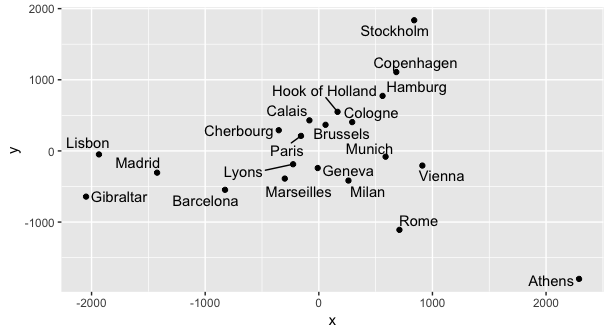
\includegraphics[scale = 0.5]{./images/europ_cities.png}
    \caption{MDS on the Eurepean cities.}
    \label{europ_cities}
\end{figure}

\indent MDS methods can be divided into two groups: \textit{Metric MDS} and
\textit{Non-metric MDS}. Metric MDS, also known as principal coordinates, use
the differences between similarities. However, Non-metric MDS states that if $a$
is more similar to $b$ than $c$, then $a$ is closer to $b$ than $c$, but the
differences between the similarities $ab$ and $ac$ do not have any 
interpretation. This thesis is focused on the Metric MDS.

\section{A historical Account}
The first decade was pioneered by the seminal work of Torgerson (1952), he 
defined the multidimensional scaling problem and provided the first metric 
solution. 

\begin{itemize}
\item Torgerson\cite{Torgerson1952} provided the first complete explication 
of a MDS method. Although Klingberg (1941) had already performed a "crude" 
MDS scaling of data concerning the degree of hostility between nations, the 
first systematic procedure for determining the MDS map of points from 
errorful interpoint distances was provided by Torgerson (1952)\cite{Torgerson1952}.

\item This process introduced three major steps:

\begin{itemize}

\item A scale of comparative distances between all pairs of stimuli is obtained 
(i.e. measured on an interval scale)

\item Distances between each pair of stimuli are located on a distance continuum.
In paired comparisons, the procedures for obtaining a scale of comparative 
distances leave the true zero point undetermined. A comparative distance is 
not a distance in the usual sense of the term, but is a distance minus an 
unknown constant. When the unknown constant is obtained, the comparative 
distances can be converted into absolute (i.e., ratio) distances. 

\item The dimensionality of the psychological space necessary to account for 
these absolute distances is determined, and the projections of stimuli on 
axes of this space are obtained.

\end{itemize}
\end{itemize}
 
\indent The second decade of work was heralded in by the innovative work of 
Shepard (1962)\cite{Shepard1962} and Kruskal (1964)\cite{Kruskal1964} on 
non-metric multidimensional scaling, and saw the highly illuminating work of 
Coombs (1964)\cite{coombs} on data theory. 

\begin{itemize}
\item This very active decade included work that focused on developing methods 
for analyzing ordinal dissimilarities data known as nonmetric MDS. This stage 
became popularized by Shepard (1962)\cite{Shepard1962} who turned "MDS from a 
data analysis procedure familiar to a few aficionados into a procedure used in 
such diverse disciplines as architecture and zoology, geography and political 
science, and psychology and business administration.". Shepard pointed out the 
idea that one could recover metric information from nonmetric information.
\end{itemize}

\indent The third decade included 25 years of developments by Takane, Young, 
and De Leeuw (1976)\cite{takane}, and by the De Leeuw and Heiser (1980)\cite{de_leeuw}. 
The trend setting work came from Carroll and Chang (1970)\cite{Carroll1970} on individual 
differences MDS. 

\begin{itemize}
\item Before this point, MDS procedures could only analyze a single matrix of 
data. Leading to the development of "individual differences"  MDS. (i.e. 
procedures that were able to simultaneously analyze a number of data matrices 
without the necessity of any type of averaging process). 

\item Carroll and Chang proposed a model for representing cognitive/perceptual 
individual differences whose psychological appeal was very high, which displayed 
individual differences in an easily assimilated and parsimonious fashion.
\end{itemize}

\indent  The fourth decade presented the development of constrained MDS and 
maximum likelihood multidimensional scaling, as exemplified by Ramsay (1982) and 
Takane (1980a, 1980b)\cite{takane}. 

\begin{itemize}
\item Constrained MDS - introduction of constraints on the parameters 
of the  model. 

\item Maximum likelihood MDS - A maturing of the data analysis technology 
usually brings a desire for an explanation of the error model involved in 
the fitting process (Ramsay 1977). 

\item This approach changes MDS from a descriptive tool into an inferential 
tool. 

\item This includes the development of significant tests to determine the 
appropriate dimensionality, appropriate MDS model, and appropriate 
error model. 

\item This approach provides confidence regions for the stimuli and with 
weighted models for subjects.         
\end{itemize}

\indent Most applications of MDS today actually serve a wide purpose, i.e. they 
are done to visualize tables of indices that can be interpreted as 
(dis)similarity data. For that purpose, MDS is highly useful as it can handle a 
vast variety of data as long as they are (dis)similarities 
(e.g., correlations, covariances, co-occurrence data, profile distances).

\section{Principal coordinates}
Given a Matrix \textbf{X} $n \times p$, one can interpret it as the matrix of $n$ 
individuals over $p$ variables. It is easy to see that the following matrix
has mean zero:

$$\mathbf{\widetilde{X}} = \Big( \mathbf{I} - \frac{1}{n} \mathbf{1}\mathbf{1'}\Big) = \mathbf{P}\mathbf{X}$$

This new matrix, $\mathbf{\widetilde{X}}$ has the same dimensions as the orginial one, but
it is centered. From this matrix, it is possible to build two square semi-positive
definite matrices: the covariance matrix \textbf{S}, defined as 
$\mathbf{\widetilde{X}'}\mathbf{\widetilde{X}}/n$ and the cross-prodructs matrix 
$Q = \mathbf{\widetilde{X}}\mathbf{\widetilde{X}'}$. This matrix can be interpred as a similarity 
matrix between the n elements. The term $ij$ is obtained as follows:

\begin{equation} \label{qij}
q_{ij} = \sum_{s=1}^{p} x_{is}x_{js} = \mathbf{x_i'} \mathbf{x_j}
\end{equation}



where $\mathbf{x_i'}$ is the i-th row from $\mathbf{\widetilde{X}}$. 
Given the scalar product formula, $\mathbf{x_i'}\mathbf{x_j} =  \mid \mathbf{x_i} \mid \mid \mathbf{x_i} \mid cos\theta_{ij}$,
if the elements i and j have similar coordinates, then $cos\theta_{ij} \simeq 1$
and $q_{ij}$ will be large. On the contrary, if the elements are very different,
then $cos \theta_{ij} \simeq 0$ and $q_{ij}$ will be small. So, 
$\mathbf{\widetilde{X}}\mathbf{\widetilde{X}'}$ can be interpreted as the similarity
matrix between the elements.

\indent The distances between elements can be deduced from the similarity matrix.
The euclidean distance between to elements is calculated in the following way:

\begin{equation} \label{dij}
d^2_{ij} = \Big ( \sum_{s=1}^{p} x_{is}- x_{js} \Big )^2 = \sum_{s=1}^{p}x_{is}^2 + \sum_{s=1}^p x_{js}^2 - 2\sum_{s=1}^{p} x_{is}x_{js}
\end{equation}

\indent This expression can be obtained directly from the matrix \textbf{Q}:

\begin{equation} \label{dfromq}
d^2_{ij} = q_{ii} + q_{jj} - 2q_{ij}
\end{equation}

\indent We have seen that given the matrix $\mathbf{\widetilde{X}}$, it is possible to
get the similarity matriz $\mathbf{Q} = \mathbf{\widetilde{X}}\mathbf{\widetilde{X}'}$
and from it, to get the distance matrix \textbf{D}. Let $diag(\mathbf{Q})$ be the
vector that contains the diagonal terms of \textbf{Q} and \textbf{1} be the vector
of ones, the matrix \textbf{D} is given by:

$$\mathbf{D} = diag(\mathbf{Q}) \mathbf{1}' + \mathbf{1}diag(\mathbf{Q})' - 2\mathbf{Q}$$

\indent The problem we are dealing with goes in the opposite direction. We want to rebuid
$\mathbf{\widetilde{X}}$ from a square distance matrix \textbf{D}, with elements
$d_{ij}^2$. The first step is to obtain \textbf{Q} and afterwards, to get 
$\mathbf{\widetilde{X}}$. \textit{Daniel Peña} develops in his book\cite{pena_libro} the theory
needed to get the solution. Here, we summarise it.

\indent The first step is to find out a way to obtain the matrix \textbf{Q} given
\textbf{D}. We can assume without loss of generality that the mean of the variables
is equal to 0. This is a consequence of the fact that the distance between two points
keeps unchanged if the variables are expressed in terms of the mean:


\begin{equation} \label{dtraslated}
d_{ij}^2 = \sum_{s = 1}^p (x_{is} - x_{js})^2 = \sum_{s=1} ^p [(x_{is} - \overline{x_s})- (x_{js} - \overline{x_s})]^2
\end{equation}

\indent The previous condition means that we are lookig for a matrix  $\mathbf{\widetilde{X}}$
such that $\mathbf{\widetilde{X}'}\mathbf{1} = 0$. It also means that $\mathbf{Q}\mathbf{1} = 0$,
i.e, the sum of all the elements of a row of \textbf{Q} is 0. Since the matrix is 
symmetric, the previous condition should state for the columns as well. 

\indent To establish this constrains, we sum up \ref{dij} at row level:

\begin{equation} \label{sumrows}
\sum_{i = 1}^n d_{ij}^2 = \sum_{i = 1}^n q_{ii} + nq_{jj} = t + nq_{jj}
\end{equation}

where $t = \sum_{i = 1}^n q_{ii} = trace(\mathbf{Q})$, and we have used that the
condition \textbf{Q}\textbf{1} = 0 implies $\sum_{i = 1}^n q_{ij} = 0$. Summing 
up the \ref{dij} at column level:

\begin{equation} \label{sumcols}
\sum_{i = 1}^n d_{ij}^2 = t + nq_{ii}
\end{equation}

\indent Summing up \ref{sumrows} we obtain:

\begin{equation} \label{doublesum}
\sum_{i = 1}^n\sum_{j = 1}^n d_{ij}^2 = 2nt
\end{equation}

\indent Replacing in \ref{dfromq} $q_{jj}$ obtained in \ref{sumrows} and $q_{ii}$
obtained in \ref{sumcols}, we have the following expression:

\begin{equation} \label{generaldij}
d_{ij}^2 = \frac{1}{n}\sum_{i = 1}^n d_{ij}^2 - \frac{t}{n} + \frac{1}{n} \sum_{j = 1}^n d_{ij}^2 -\frac{t}{n} -2q_{ij}
\end{equation}

\indent Let $d_{i.}^2 = \frac{1}{n}\sum_{j = 1}^n d_{ij}^2$ and $d_{.j}^2 = \frac{1}{n}\sum_{i=1}^n d_{ij}^2$ 
be the row-mean and column-mean. Using \ref{doublesum}, we have that:

\begin{equation} \label{dmeans}
d_{ij}^2 = d_{i.}^2 + d_{.j}^2 - d_{..}^2-2q_{ij}
\end{equation}

where $d_{..}$ if the mean of all the elements of \textbf{D}, gven be:

$$d_{..}^2 = \frac{1}{n^2}\sum \sum d_{ij}^2$$

\indent Finally, from \ref{dmeans} we get the following expression:

\begin{equation} \label{qij2}
q_{ij} = -\frac{1}{2}(d_{ij}^2 - d_{i.}^2 - d_{.j}^2 + d_{..}^2)
\end{equation}

\indent The previous expression shows how to build the matrix of similarities \textbf{Q}
from the distance matrix \textbf{D}.

\indent The next step is to obtain the matrix \textbf{X} given the matrix \textbf{Q}.
Let's supose that the similarity matrix es positive definite of range $p$, it can
be represented by 

$$\mathbf{Q} = \mathbf{V}\mathbf{\Lambda}\mathbf{V'}$$

where $\mathbf{V}$ is a $n \times p$ matrix that contains the eigenvectors with
eigenvalues not nulls of \textbf{Q}, $\mathbf{\Lambda}$ is a diagonal matrix 
$p \times p$ that contains the eigenvalues.

\indent Re-writing the previous expression, we obtain:

\begin{equation} \label{generalQ}
\mathbf{Q} = (\mathbf{V}\mathbf{\Lambda}^{1/2})(\mathbf{\Lambda}^{1/2}\mathbf{V'})
\end{equation}

Getting:

$$Y = \mathbf{V}\mathbf{\Lambda}^{1/2}$$

we have obtained a matrix with dimesions $n \times p$ with $p$ uncorrelated
variables that reproduces the initial metric. It is important to notice that if 
one starts from \textbf{X} (i.e \textbf{X} is known) and calculates from these
variables the distance matrix in \ref{dij} and after that it is applied
the method explained, the matrix obtained is not the same as \textbf{X}, but
its principal components. This happens since the distance between elements
does not change if:

\begin{itemize}
\item The mean values are modified
\item Poits are rotated, i.e, multiplications by orthogonal matrices
\end{itemize}

\indent By \ref{dfromq}, the distance is a function of the terms of the 
similarity matrix \textbf{Q} and this matrix is invariant given any rotations of
the variables:

$$\mathbf{Q} = \mathbf{\widetilde{X}} \mathbf{\widetilde{X'}} = \mathbf{\widetilde{X}} \mathbf{A} \mathbf{A'}\mathbf{\widetilde{X'}}$$

for any orthogonal \textbf{A} matrix. The matrix \textbf{Q} anly contains 
information about the space generated by the variables \textbf{X}. Any rotation
keeps the distance unchaged. As a consequence, any rotation of the original 
variables could be a valid solution.


\section{Building principal coordinates}
In general, the distance matrix is not compatible with an euclidean metric but
usually the similarity matrix obtained from it has $p$ postive eigenvalues  
and greater than the other ones. If the rest $n-p$ not null eigenvalues 
are much less than the other ones, it is possible to obtain an (approximated)
representation using the $p$ eigenvectors associated with the first $p$
eigenvalues of the similarity matrix. 

\indent Let's supose that we have a square distance matrix \textbf{D}. The
process to obtain the \textit{principal coordinates} is:

\begin{enumerate}
\item Build the matrix $\mathbf{Q = - \frac{1}{2} PDP}$ of cross-products.
\item Obtain the eigenvalues of \textbf{Q}. Take the $r$ greatest eigenvalues. 
Since $\mathbf{P1=0}$, where \textbf{1} is a vector of ones, $range(\mathbf{Q})=n-1$,
being the vector \textbf{1} an eigenvector with eigenvalue 0.
\item Obtain the coordinates of the individuals in the variables $\mathbf{v_i}\sqrt{\lambda_i}$,
where $\lambda_i$ is an eigenvalue of \textbf{Q} and $\mathbf{v_i}$ is the
associated unitary eigenvector. This implies that \textbf{Q} is apporximated by:

$$\mathbf{Q} \approx (\mathbf{V_r \Lambda}^{1/2})(\mathbf{\Lambda_r}^{1/2} \mathbf{V_r'})$$

\item Take as coordinates of the points the following variables:
$$\mathbf{Y_r} = \mathbf{V_r}\mathbf{\Lambda_r}^{1/2}$$
\end{enumerate}

\indent The method can also be applied if the initial information is not a distance matrix
but a similarity matrix. A \textit{similarity function} between two element $i$
and $j$ $s_ij$ is defined as:

\begin{itemize}
\item $s_ii = 1$
\item $0 \leq s_{ij} \leq 1$
\item $s_{ij} = s_{ji}$
\end{itemize}

If the initial information is \textbf{Q}, a similariy matrix, then $q_{ii} = 1$,
$q_{ij} = q_{ji}$ and $0 \leq q_{ij} \leq 1$. The assiciated distance matrix 
(by \ref{dfromq}):

$$d_{ij}^2 = q_{ii} + q_{jj} - 2q_{qij} = 2(1-q_{ij})$$

and it is easy to see that $\sqrt{2(1-q_{ij})}$ is a distance and it verifies
the triangle inequality.


\section{Procrustes transformation}
As we have mentioned, the MDS solution is not unique. Since rotation, translation,
reflections and dilations are distance-preserving functions, one can found two
different MDS configurations for the same set of data. How is it possible to
align both solutions? One example of it can be found in figure \ref{twosol}.

\begin{figure}[ht]
    \centering
    \subfloat[]{{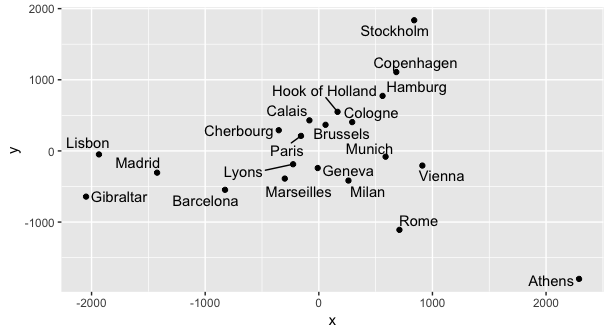
\includegraphics[width=8cm]{./images/europ_cities.png} }}%
    \qquad
    \subfloat[]{{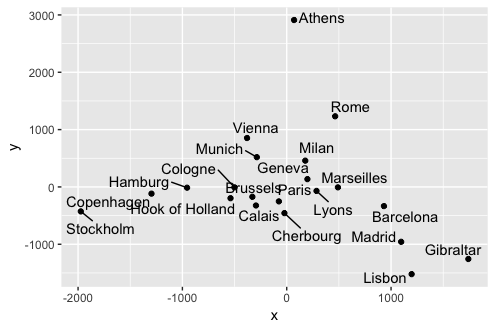
\includegraphics[width=8cm]{./images/europ_cities_rot.png} }}%
    \caption{Two different solutions of MDS}%
    \label{twosol}%
\end{figure}


\indent The Procrustes problem is concern with fitting a configuration (testee)
to another (target) as closly as possible. In the simple case, both 
configurations have the same dimensionality and the same number of points, which
can be brought into 1-1 correspondence by substantive considerations. Under
orthogonal transformations, the testee can be rotated and reflected arbitrarily
in an effort to fit it to the target. In addition to such rigid motions, one 
may also allow for dilations and for shifts.

\indent \textit{Ingwer Borg} and \textit{Patrik Groenen} detail all the steps 
needed to obtain the solution\cite{BorgGroenen2005}. This is out of the scope of 
this thesis. However, sicen it has been a repeatdly used tool, we briefly 
summarise it. 

\indent Let \textbf{A}, and \textbf{B} be two different MDS configurations for
the same set of data. Without loss of generality, let's suposo that the target 
is \textbf{A} and the testee is \textbf{B}. One wants to obtain $s$, \textbf{T}
and $t$ such that:

$$A = s \mathbf{B} \mathbf{T} + \mathbf{1t}'$$

where \textbf{T} is an orthogonal matrix. As mentioned before, \textit{Ingwer Borg} 
and \textit{Patrik Groenen} develop all the theory\cite{BorgGroenen2005} that 
allows to get these parameters.

\section{Multidimensional Scaling with \textsf{R}}

All the algorithms have been coded in \textsf{R}, since it has a widely statistics
pckages already implemented. We have used two packages for developing our MDS
approaches:

\begin{itemize}
\item Package: \textsf{stats}. From this one we have used the fucntion 
\textsf{cmdscale} to do the MDS. The output of this function is:
\begin{itemize}
\item The new coordinates for the individuals.
\item All the eigenvalues found.
\end{itemize}
\item Package: \textsf{MCMCpack}. From this one we have used the fucntion 
\textsf{cmdscale} to do the Procrustes transformation. The output of 
this function is:
\begin{itemize}
\item The dilation coeficient $s$.
\item The orthogonal matrix \textbf{T}.
\item The translation vector \textbf{t}.
\end{itemize}
\end{itemize}

\chapter{Divde and Conquer Multidimensional Scaling}


\chapter{Fast Multidimensional Scaling}


\chapter{Multidimensional Scaling based on Gower interpolation formula}

\chapter{Simulation study}


\chapter{Conclusions}

\bibliographystyle{unsrt}
\bibliography{bibliography.bib}


\appendix 

\chapter{masblablabl}
blabla
\end{document}


% Notacion:
% Matrices: mayusculas y negritas
% Vectores: minusculas y negritas
% constantes: minusculas y normal

% Mencionar a Roger
% Ejemplo de un MDS con dos soluciones (rota una solucion)
% Añadir los artículos que Pedro me pasó para el capitulo de Gower
